% Schematic representation of corona poling
% From NLO of organic molecules and polymers, Singh/Miyata.
% Author: Orlando Torres (2016)
\documentclass{standalone}
\usepackage{amsmath} % Required for \varPsi below
\usepackage{tikz,pgfplots}
\usetikzlibrary{calc}
\usetikzlibrary{patterns}
\tikzset{>=latex}
\begin{document}
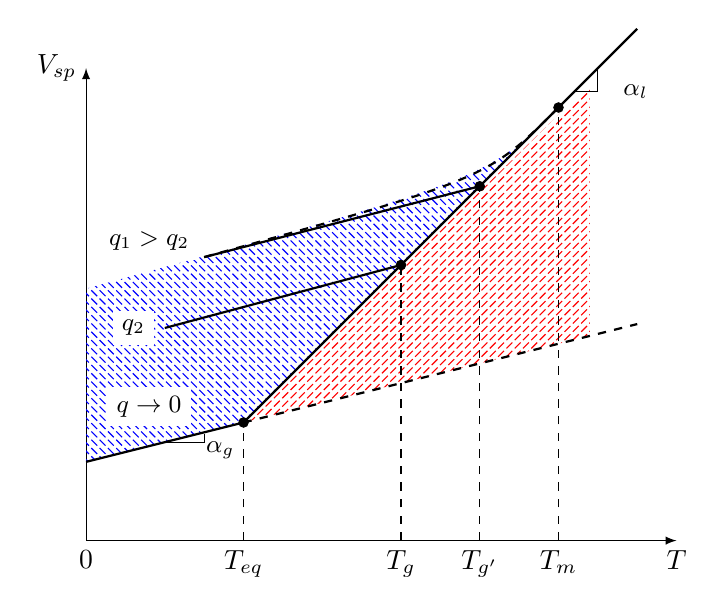
\begin{tikzpicture}

\coordinate (sg) at (5.9, 3);
\coordinate (sa) at (5.9, 3);

% horizontal axis
%\node [draw=blue,rotate=0,anchor=north,outer sep=-4pt] at (-0.3,4.3) {V};
\draw[->] (0,0) -- (7.5,0) node[anchor=north] {$T$};
% labels
\draw	(0,0) node[anchor=north] {0}
		(2.0,0) node[anchor=north] {$T_{eq}$}
		(4.0,0) node[anchor=north] {$T_{g}$}
		(5.0,0) node[anchor=north] {$T_{g'}$}
		(6.0,0) node[anchor=north] {$T_m$};
% ranges


% vertical axis
\draw[->] (0,0) -- (0,6) node[anchor=east] {$V_{sp}$};
% labels
\draw	(1.4,1.15) node[anchor=west] {\small $\alpha_g$}
		(6.7,5.7) node[anchor=west] {\small $\alpha_l$}
		%(0,2.5) node[anchor=east] {$T_p$}
		%(0.8,1.6) node[anchor=west,fill=white] {$q \rightarrow 0$}
		%(0,3.4) node[anchor=east] {$V_p$}
		%(0,3.2) node[anchor=south] {-}
		%(0,3.0) node[anchor=east] {$i_p$}
		%(0,2.8) node[anchor=south] {-}
		%(0,2.0) node[anchor=east] {$i_t$}
		%(0,1.8) node[anchor=south] {-}
		;

%fill zone
\fill [draw=none, pattern=north west lines, pattern color=blue, dashed] (0.0,1.0) -- (2.0,1.5) -- (6.0,5.5) .. controls (5.1,4.6) .. (0,3.2)  -- cycle;
\fill [draw=none, pattern=north east lines, pattern color=red,dashed] (2.0,1.5) -- (6.4,2.6) -- (6.4,5.8)  -- cycle;

\draw[thick,dashed,color=black] (1.5,3.6) .. controls (5.1,4.6)  .. (6.0,5.5);
% Vertical lines
\draw[dashed] (2.0,0) -- (2.0,1.5);
\draw[dashed] (4.0,0) -- (4.0,3.5);
\draw[dashed] (5.0,0) -- (5.0,4.5);
\draw[dashed] (6.0,0) -- (6.0,5.4);

%q->0
\draw[thick] (0.0,1.0) -- (2.0,1.5);
%q->0 cont.
\draw[thick,dashed] (2.0,1.5) -- (7.0,2.75);
%q->0 at alpha_l
%q->0
\draw[thick] (2.0,1.5) -- (7.0,6.5);

%q->2
\draw[thick] (1.5,3.6) -- (5,4.5);

%q->1

%and (3.5,3.4)

\draw[thick] (1,2.7) -- (4.0,3.5);

 \node [shape=circle, color=black, fill=black, inner sep=1.2, draw]
    (substrate) at (2.0,1.5) {};
 \node [shape=circle, color=black, fill=black, inner sep=1.2, draw]
    (substrate) at (4.0,3.5) {};
 \node [shape=circle, color=black, fill=black, inner sep=1.2, draw]
    (substrate) at (5.0,4.5) {};
 \node [shape=circle, color=black, fill=black, inner sep=1.2, draw]
    (substrate) at (6.0,5.5) {};



%angles
\draw (1,1.25) -- (1.5,1.25) -- (1.5,1.35);
\draw (6.2,5.7) -- (6.5,5.7) -- (6.5,6.0);

\node [shape=rectangle, minimum width=10, minimum height=6,  fill=white, draw=none] (nq) at (0.8,1.7) {\small$ q \rightarrow 0$};
\node [shape=rectangle, minimum width=10, minimum height=6,  fill=white, draw=none] (nq) at (0.6,2.7) {\small $q_2$};
\node [shape=rectangle, minimum width=10, minimum height=6,  fill=white, draw=none] (nq) at (0.8,3.8) {\small $q_1>q_2$};

%\draw (sa) node (sa) at +(0.4, -0.55) {$T(t)$};

%\draw (1,1.5) node {$U_s$}; %label
%Y tick marks
%\foreach \x in {0,...,6}
%     		\draw (\x,1pt) -- (\x,-3pt)
%			node[anchor=north] {\x};
%    	\foreach \y in {0,...,4}
%     		\draw (1pt,\y) -- (-3pt,\y) 
%     			node[anchor=east] {\y}; 
% Psis
%\draw[thick,dashed] (0,3) -- (2,3) parabola[bend at end] (6,1);
%\draw (2.5,3) node {$\varPsi_s$}; %label

\end{tikzpicture}

\end{document}